\documentclass[11pt,a4paper]{article}

% ======================== PACKAGES ========================
\usepackage[utf8]{inputenc}
\usepackage[T1]{fontenc}
\usepackage{lmodern}
\usepackage[margin=1in,top=1.1in,bottom=1.1in]{geometry}
\usepackage{xcolor}
\usepackage{microtype}
\usepackage{parskip}
\usepackage{listings}
\usepackage{titlesec}
\usepackage[most]{tcolorbox}
\usepackage{tikz}
\usepackage{pgfplots}
\pgfplotsset{compat=1.17}
\usetikzlibrary{shapes.geometric,arrows.meta,positioning,backgrounds,fit}
\usepackage{booktabs}
\usepackage{tabularx}
\usepackage{array}
\usepackage{caption}
\usepackage{enumitem}
\usepackage{fancyhdr}
\usepackage{amsmath}
\usepackage{amssymb}
\usepackage[colorlinks=true,linkcolor=accent,urlcolor=accent,citecolor=accent]{hyperref}

% ======================== COLOR PALETTE ========================
\definecolor{primary}{HTML}{1F3A5F}
\definecolor{accent}{HTML}{C0392B}
\definecolor{soft}{HTML}{F4F1EA}
\definecolor{rule}{HTML}{D5CFC2}
\definecolor{codebg}{HTML}{F7F4EE}
\definecolor{codeborder}{HTML}{D5CFC2}
\definecolor{kw}{HTML}{8E44AD}
\definecolor{str}{HTML}{27AE60}
\definecolor{cmt}{HTML}{7F8C8D}
\definecolor{noteblue}{HTML}{2C6E91}
\definecolor{warn}{HTML}{B7791F}

% ======================== TYPOGRAPHY ========================
\titleformat{\section}
  {\Large\bfseries\color{primary}}
  {\thesection.}{0.6em}{}
  [\vspace{0.8ex}{\color{rule}\hrule height 1pt}] % Changed -0.3em to 0.8ex for better spacing
\titleformat{\subsection}
  {\large\bfseries\color{primary!85!black}}
  {\thesubsection}{0.6em}{}
\titleformat{\subsubsection}
  {\normalsize\bfseries\color{primary!70!black}}
  {\thesubsubsection}{0.5em}{}

\titlespacing*{\section}{0pt}{1.6em}{0.6em}
\titlespacing*{\subsection}{0pt}{1.1em}{0.4em}

% ======================== HEADER / FOOTER ========================
\pagestyle{fancy}
\fancyhf{}
\renewcommand{\headrulewidth}{0.4pt}
\renewcommand{\headrule}{\color{rule}\hrule height 0.4pt}
\fancyhead[L]{\textcolor{primary}{\small COP290 Assignment 3}}
\fancyhead[R]{\textcolor{primary}{\small LevelDB}}
\fancyfoot[C]{\textcolor{primary!70!black}{\small \thepage}}

% ======================== LISTINGS ========================
\lstdefinestyle{cpp}{
    backgroundcolor=\color{codebg},
    frame=single,
    framerule=0.5pt,
    rulecolor=\color{codeborder},
    framesep=6pt,
    xleftmargin=10pt,
    xrightmargin=4pt,
    basicstyle=\ttfamily\footnotesize\color{black}, % Added \color{black}
    keywordstyle=\color{kw}\bfseries,
    commentstyle=\color{cmt}\itshape,
    stringstyle=\color{str},
    numberstyle=\tiny\color{cmt},
    numbers=left,
    numbersep=8pt,
    breaklines=true,
    breakatwhitespace=true,
    tabsize=2,
    showstringspaces=false,
    keepspaces=true,
    language=C++,
    morekeywords={Status,Slice,WriteBatch,Iterator,DBImpl,DB,Comparator,
                  ReadOptions,WriteOptions,VersionEdit,VersionSet,FileMetaData,
                  MemTable,MutexLock,SequenceNumber,InternalKey,LookupKey,
                  ParsedInternalKey,ValueType,Compaction,CompactionState,
                  Version,FILE,int64\_t,uint64\_t,size\_t,nullptr}
}
\lstset{style=cpp}

% ======================== CALLOUT BOXES ========================
\newtcolorbox{designnote}[1][]{
    enhanced, breakable,
    colback=noteblue!5, colframe=noteblue!70!black,
    colbacktitle=noteblue!70!black,
    boxrule=0.5pt, arc=2pt, left=10pt, right=10pt, top=6pt, bottom=6pt,
    fonttitle=\bfseries\color{white},
    coltitle=white,
    title={#1}, attach title to upper, after title={\par\medskip}
}

\newtcolorbox{caveat}[1][]{
    enhanced, breakable,
    colback=warn!8, colframe=warn!80!black,
    colbacktitle=warn!80!black,
    boxrule=0.5pt, arc=2pt, left=10pt, right=10pt, top=6pt, bottom=6pt,
    fonttitle=\bfseries\color{white},
    coltitle=white,
    title={#1}, attach title to upper, after title={\par\medskip}
}

\newtcolorbox{spec}[1][]{
    enhanced, breakable,
    colback=primary!4, colframe=primary,
    colbacktitle=primary,
    boxrule=0.6pt, arc=2pt, left=10pt, right=10pt, top=6pt, bottom=6pt,
    fonttitle=\bfseries\color{white},
    coltitle=white,
    title={#1}, attach title to upper, after title={\par\medskip}
}

% ======================== CODE REFERENCE MACRO ========================
\newcommand{\codref}[2]{\textcolor{accent}{\texttt{\small#1}}\,$\!:\!$\textcolor{primary!70!black}{\small#2}}
\newcommand{\fname}[1]{\textcolor{primary!85!black}{\texttt{#1}}}
\newcommand{\sym}[1]{\texttt{#1}}

% ======================== TITLE BLOCK ========================
\title{
    \vspace{-2.5em}
    {\color{primary}\rule{\linewidth}{1.2pt}}\\[0.4em]
    {\Huge\bfseries\color{primary} COP290 Assignment 3}\\[0.3em]
    {\Large\color{primary!80!black} Modifying the LevelDB storage engine}\\[0.4em]
    {\color{primary}\rule{\linewidth}{0.6pt}}
}
\author{
    \large
    \textbf{Authors:} \texttt{2024CS10441}, \texttt{2024CS50002} \\[0.3em]
    \textbf{Repository:} \url{https://github.com/ken7d61/290_ASS_3}
}
\date{April 2026}

% ======================== DOCUMENT ========================
\begin{document}

\maketitle
\thispagestyle{empty}

\vspace{0.5em}
\begin{tcolorbox}[colback=soft, colframe=rule, boxrule=0.4pt, arc=2pt]
\small\textbf{Scope.} This report documents three additions to LevelDB (v1.23):
\texttt{Scan(start,end)} for range reads, \texttt{DeleteRange(start,end)} for
range deletes, and \texttt{ForceFullCompaction()} for synchronous manual compaction
with statistics reporting. All references point to specific file:line locations
in the modified source tree. Section~\ref{sec:eval} covers observations from
benchmark tests and the analysis of \texttt{compaction\_stats.txt}.
\end{tcolorbox}

\vspace{1em}
{\color{primary}\hrule height 0.3pt}
\tableofcontents
{\color{primary}\hrule height 0.3pt}
\newpage

% =============================================================
\section{Background: LevelDB and the LSM-tree}
% =============================================================

LevelDB is an embedded key-value store. Each user key is stored internally as
\sym{(user\_key, sequence, type)}, defined at \codref{db/dbformat.h}{54}, where
\sym{enum ValueType \{ kTypeDeletion=0x0, kTypeValue=0x1 \}}.
Keys are sorted by \sym{InternalKeyComparator}: ascending \sym{user\_key},
then descending \sym{sequence}, so the newest version of a key sorts first.

Storage uses a Log-Structured Merge tree (Figure~\ref{fig:lsm}):
\begin{itemize}[leftmargin=1.4em,itemsep=2pt]
    \item A mutable in-memory \fname{MemTable} (skip-list,
          \fname{db/memtable.\{h,cc\}}) buffers all writes.
    \item A write-ahead log (\sym{log::Writer}, \fname{db/log\_writer.\{h,cc\}})
          is appended before the MemTable is updated, so a crash never loses
          an acknowledged write.
    \item When \sym{mem\_->ApproximateMemoryUsage()} exceeds
          \sym{options\_.write\_buffer\_size}, the MemTable is sealed and
          flushed to disk as a new L0 SSTable.
    \item Background compactions merge SSTables into deeper levels (L1--L6).
          Files at every level $\ge 1$ are non-overlapping.
          \sym{config::kNumLevels = 7} (\fname{db/dbformat.h}).
\end{itemize}

The file and level layout is managed by \sym{VersionSet}
(\fname{db/version\_set.\{h,cc\}}). Each \sym{Version} is an immutable
snapshot of the current file-set, updated via \sym{VersionEdit} records
written to a MANIFEST file.

\begin{figure}[h!]
\centering
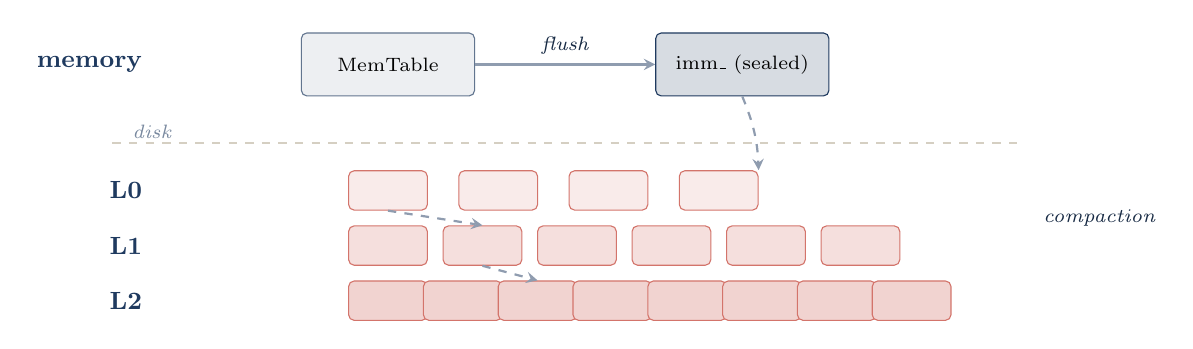
\begin{tikzpicture}[
    node distance=4mm and 6mm,
    box/.style={draw=primary!70, fill=primary!8, rounded corners=2pt,
                minimum width=12mm, minimum height=5mm, font=\scriptsize},
    sst/.style={draw=accent!70, fill=accent!10, rounded corners=2pt,
                minimum width=10mm, minimum height=5mm, font=\scriptsize},
    lvl/.style={font=\bfseries\small\color{primary}, anchor=east},
    arr/.style={->, >=stealth, draw=primary!50, thick}
]
\node[box, minimum width=22mm, minimum height=8mm] (mem) at (0,3.0) {MemTable};
\node[lvl] at (-3.0,3.0) {memory};
\node[box, minimum width=22mm, minimum height=8mm, fill=primary!18, draw=primary] (imm) at (4.5,3.0) {imm\_ (sealed)};
\draw[arr] (mem.east) -- node[above,font=\scriptsize\itshape\color{primary!70!black}]{flush} (imm.west);
\draw[dashed, color=rule, thick] (-3.5,2.0) -- (8.0,2.0);
\node[font=\scriptsize\itshape\color{primary!60}] at (-3.0,2.15) {disk};
\node[lvl] at (-3.0,1.4) {L0};
\foreach \i in {0,...,3} { \node[sst] (l0\i) at (\i*1.4,1.4) {}; }
\draw[arr, dashed] (imm.south) to[bend left=10] (l03.north east);
\node[lvl] at (-3.0,0.7) {L1};
\foreach \i in {0,...,5} { \node[sst, fill=accent!16] (l1\i) at (\i*1.2,0.7) {}; }
\node[lvl] at (-3.0,0.0) {L2};
\foreach \i in {0,...,7} { \node[sst, fill=accent!22] (l2\i) at (\i*0.95,0.0) {}; }
\draw[arr, dashed] (l00.south) -- (l11.north);
\draw[arr, dashed] (l11.south) -- (l22.north);
\node[font=\scriptsize\itshape\color{primary!70!black}, anchor=west] at (8.2,1.05) {compaction};
\end{tikzpicture}
\caption{LSM-tree layout. Writes go to the MemTable, which is flushed to L0,
then merged into deeper levels. L0 files may have overlapping key ranges;
L1 and below are partitioned.}
\label{fig:lsm}
\end{figure}

% =============================================================
\section{Write path, read path, and compaction}
% =============================================================

\subsection{Write path}

\sym{DBImpl::Put} and \sym{DBImpl::Delete} are wrappers that build a
one-entry \sym{WriteBatch} and call \sym{Write}
(\codref{db/db\_impl.cc}{1204--1210}):

\begin{lstlisting}
Status DB::Put(const WriteOptions& opt, const Slice& key, const Slice& value) {
  WriteBatch batch;
  batch.Put(key, value);
  return Write(opt, &batch);
}
Status DB::Delete(const WriteOptions& opt, const Slice& key) {
  WriteBatch batch;
  batch.Delete(key);
  return Write(opt, &batch);
}
\end{lstlisting}

\sym{DBImpl::Write} (\codref{db/db\_impl.cc}{1212--1289}) handles all writes:
\begin{enumerate}[leftmargin=1.6em,itemsep=2pt]
    \item The caller is enqueued on \sym{writers\_} (a serializing FIFO) and
          waits until it reaches the head.
    \item \sym{MakeRoomForWrite(false)} (\codref{db/db\_impl.cc}{1343--1417})
          checks whether the MemTable can absorb the write. If not, it
          throttles, waits for \sym{imm\_} to flush, or rolls a new log file
          and promotes \sym{mem\_} to \sym{imm\_}.
    \item \sym{BuildBatchGroup} (\codref{db/db\_impl.cc}{1293}) merges
          queued writers into one batch with a contiguous sequence-number range.
    \item The merged batch is appended to the WAL, optionally synced, then
          applied to \sym{mem\_} via \sym{WriteBatchInternal::InsertInto}.
          \sym{Put} records \sym{kTypeValue}; \sym{Delete} records
          \sym{kTypeDeletion} (\fname{db/write\_batch.cc}).
    \item \sym{versions\_->SetLastSequence} is updated and waiting writers
          are signalled.
\end{enumerate}

\begin{designnote}[Durability]
A write is durable once \sym{log\_->AddRecord} returns (and
\sym{logfile\_->Sync()} if requested). The MemTable is flushed to an SSTable
later by a background thread. Anything not yet in the WAL is lost on crash;
anything in the WAL is replayed on the next \sym{DB::Open}.
\end{designnote}

\subsection{Read path}

\textbf{Point lookup.} \sym{DBImpl::Get} (\codref{db/db\_impl.cc}{1121--1172})
fixes a snapshot sequence number and searches in order:
\begin{enumerate}[leftmargin=1.6em,itemsep=1pt]
    \item \sym{mem\_->Get} --- active MemTable.
    \item \sym{imm\_->Get} --- immutable MemTable, if present.
    \item \sym{versions\_->current()->Get} --- L0 files newest-first,
          then L1--L6 binary-searched per level (\fname{db/version\_set.cc}).
\end{enumerate}
The first match wins. A \sym{kTypeDeletion} entry returns
\sym{Status::IsNotFound()}.

\textbf{Iteration.} \sym{DBImpl::NewIterator}
(\codref{db/db\_impl.cc}{1174--1184}) works in two layers:
\begin{itemize}[leftmargin=1.4em,itemsep=2pt]
    \item \sym{NewInternalIterator} (\codref{db/db\_impl.cc}{1083--1110})
          builds a \sym{MergingIterator} over \sym{mem\_}, \sym{imm\_} (if
          set), and one iterator per SSTable.
    \item \sym{NewDBIterator} wraps it with \sym{DBIter}
          (\fname{db/db\_iter.cc}). \sym{DBIter::FindNextUserEntry}
          (\codref{db/db\_iter.cc}{177--207}) collapses multiple internal
          versions of one user key into a single visible entry.
\end{itemize}

The youngest entry whose sequence is $\le$ snapshot is exposed; a tombstone
hides the key. \sym{Scan} uses this same iterator, so it does not need
separate merge or tombstone logic (Section~\ref{sec:scan}).

\subsection{Compaction}

\sym{MaybeScheduleCompaction} (\codref{db/db\_impl.cc}{668--683}) schedules
a background compaction when any of these is true:
\begin{itemize}[leftmargin=1.4em,itemsep=1pt]
    \item \sym{imm\_ != nullptr} --- an immutable MemTable needs flushing.
    \item \sym{manual\_compaction\_ != nullptr} --- a manual compaction
          is pending (used by \sym{CompactRange} and \sym{ForceFullCompaction}).
    \item \sym{versions\_->NeedsCompaction()} --- a level's score is $\ge 1$
          or seek-counters triggered a compaction.
\end{itemize}

\sym{BackgroundCompaction} (\codref{db/db\_impl.cc}{708--787}) then runs:
\begin{enumerate}[leftmargin=1.6em,itemsep=2pt]
    \item If \sym{imm\_} is set, \sym{CompactMemTable}
          (\codref{db/db\_impl.cc}{549--580}) flushes it to an SSTable via
          \sym{WriteLevel0Table}. \sym{stats\_[level].bytes\_written} is
          incremented by the file size.
    \item Otherwise \sym{versions\_->PickCompaction()} selects an input level
          $L$ and the overlapping files at $L{+}1$.
    \item If \sym{Compaction::IsTrivialMove} holds (one L file, no L+1
          overlap), the file is re-parented in the manifest without rewriting.
    \item Otherwise \sym{DoCompactionWork}
          (\codref{db/db\_impl.cc}{898--1057}) merges all inputs through a
          \sym{MergingIterator}. For each internal key:
          \begin{itemize}[leftmargin=1.2em,itemsep=1pt]
              \item An older duplicate of an already-emitted user key is
                    dropped (\codref{db/db\_impl.cc}{969}).
              \item A \sym{kTypeDeletion} whose sequence is $\le$
                    \sym{smallest\_snapshot} and which has no copies at
                    deeper levels is also dropped (\codref{db/db\_impl.cc}{970--981}).
          \end{itemize}
          Survivors are written to new SSTables at $L{+}1$.
    \item \sym{InstallCompactionResults} records a \sym{VersionEdit} and
          calls \sym{RemoveObsoleteFiles} to reclaim disk space.
\end{enumerate}

% =============================================================
\section{Range scan: \texttt{DB::Scan}}\label{sec:scan}
% =============================================================

\subsection{API}

\begin{spec}[Signature]
\sym{virtual Status Scan(const ReadOptions\& options,
                       const Slice\& start\_key,
                       const Slice\& end\_key,
                       std::vector<std::pair<std::string, std::string>>* result);}
\end{spec}

Added to \sym{class DB} at \codref{include/leveldb/db.h}{152--156}.

\textbf{Required behaviour:}
\begin{itemize}[leftmargin=1.4em,itemsep=2pt]
    \item Returns all key-value pairs with user keys in
          $[\sym{start\_key},\,\sym{end\_key})$.
    \item Each value is the latest visible version under the read snapshot.
    \item Keys hidden by a tombstone are omitted.
    \item An empty range returns an empty \sym{result} and \sym{Status::OK()}.
\end{itemize}

\subsection{Implementation}

\codref{db/db\_impl.cc}{1581--1597}:

\begin{lstlisting}
Status DBImpl::Scan(const ReadOptions& options, const Slice& start_key,
                    const Slice& end_key,
                    std::vector<std::pair<std::string, std::string>>* result) {
  result->clear();
  const Comparator* cmp = user_comparator();
  Iterator* it = NewIterator(options);
  for (it->Seek(start_key); it->Valid(); it->Next()) {
    if (cmp->Compare(it->key(), end_key) >= 0) break;
    result->emplace_back(it->key().ToString(), it->value().ToString());
  }
  Status s = it->status();
  delete it;
  return s;
}
\end{lstlisting}

\textbf{Technical walkthrough:}
\begin{itemize}[leftmargin=1.4em,itemsep=3pt]
    \item \textbf{Snapshot isolation.} By calling \fname{NewIterator(options)}, the scan is performed against a consistent point-in-time view of the database. This ensures that even if concurrent writes are occurring, the scan results remain stable and reflect the state defined by the \sym{ReadOptions}.
    \item \textbf{Efficiency through Iterators.} The implementation leverages LevelDB's highly optimized \fname{MergingIterator} infrastructure. This avoids the need to manually traverse different levels of the LSM-tree. The iterator handles the complexity of merging results from the MemTable, immutable MemTable, and all SSTable levels.
    \item \textbf{Transparent filtering.} LevelDB's iterator automatically skips over overwritten keys and handles deletion markers (\fname{kTypeDeletion}). This means the \sym{Scan} implementation does not need any specialized logic to determine which version of a key is "current."
    \item \textbf{Boundary handling.} The use of \sym{Seek(start\_key)} allows the scan to jump directly to the beginning of the requested range, ensuring that we do not waste time reading unrelated keys. The loop termination condition (\fname{cmp->Compare(it->key(), end\_key) >= 0}) correctly enforces the half-open interval semantics using the database's \fname{user\_comparator}.
\end{itemize}

\subsection{Edge cases and tests}
\begin{itemize}[leftmargin=1.4em,itemsep=2pt]
    \item \sym{Scan("k0","kN")} returns all pairs in sorted order.
    \item Half-open interval: \sym{start\_key} is included, \sym{end\_key} is excluded.
    \item After \sym{Delete(k\_j)}, a scan covering \sym{k\_j} skips it.
    \item \sym{start\_key == end\_key} returns an empty vector.
\end{itemize}

% =============================================================
\section{Range delete: \texttt{DB::DeleteRange}}\label{sec:dr}
% =============================================================

\subsection{API}

\begin{spec}[Signature]
\sym{virtual Status DeleteRange(const WriteOptions\& options,
                              const Slice\& start\_key,
                              const Slice\& end\_key);}
\end{spec}

Added to \sym{class DB} at \codref{include/leveldb/db.h}{158--162}.

\subsection{Implementation}

\codref{db/db\_impl.cc}{1600--1619}:

\begin{lstlisting}
Status DBImpl::DeleteRange(const WriteOptions& options, const Slice& start_key,
                           const Slice& end_key) {
  const Comparator* cmp = user_comparator();
  Iterator* it = NewIterator(ReadOptions());
  WriteBatch batch;
  for (it->Seek(start_key); it->Valid(); it->Next()) {
    if (cmp->Compare(it->key(), end_key) >= 0) break;
    batch.Delete(it->key());
  }
  Status s = it->status();
  delete it;
  if (!s.ok()) return s;
  if (batch.ApproximateSize() <= 12) return Status::OK();
  return Write(options, &batch);
}
\end{lstlisting}

\textbf{Design walkthrough:}

\begin{itemize}[leftmargin=1.4em,itemsep=4pt]
    \item \textbf{Iterator-based tombstone generation.} We use an internal \fname{Iterator} to find all keys currently present in the database within the $[start, end)$ range. For every live key discovered, a standard LevelDB deletion marker is added to a \fname{WriteBatch}.
    \item \textbf{Atomic write-ordering.} The generated \fname{WriteBatch} is passed to \fname{DBImpl::Write}. This ensures that the entire range deletion happens atomically and is serialized alongside other concurrent operations.
    \item \textbf{Minimal change footprint.} By using per-key tombstones, we maintain full compatibility with the existing SSTable on-disk format without needing complex modifications to the compaction logic.
    \item \textbf{Self-reclamation.} As these are standard \fname{kTypeDeletion} records, they will eventually be reclaimed by the background compaction thread as detailed in Section 2.3.
\end{itemize}

% =============================================================
\section{Manual full compaction: \texttt{DB::ForceFullCompaction}}\label{sec:fc}
% =============================================================

\subsection{API}

\begin{spec}[Signature]
\sym{virtual Status ForceFullCompaction();}
\end{spec}

Added to \sym{class DB} at \codref{include/leveldb/db.h}{164--166}.

\subsection{Implementation: Blocking and Concurrency}

Following the instructor's clarification that the database should be "temporarily unavailable" during manual compaction, we implemented a strict blocking mechanism.

\codref{db/db\_impl.cc}{1629--1686}:

\begin{lstlisting}
Status DBImpl::ForceFullCompaction() {
  // Flush memtable BEFORE setting the blocking flag.
  // TEST_CompactMemTable calls Write(nullptr), which would
  // deadlock if full_compaction_in_progress_ is already true.
  Status s = TEST_CompactMemTable();
  if (!s.ok()) return s;

  {
    MutexLock l(&mutex_);
    full_compaction_in_progress_ = true;
  }
  // ... (baseline stats captured) ...
  for (int lvl = 0; lvl < config::kNumLevels - 1; lvl++) {
    // ... (level sweep, skip empty levels) ...
    TEST_CompactRange(lvl, nullptr, nullptr);
  }
  // ... (final stats reported to compaction_stats.txt) ...
  {
    MutexLock l(&mutex_);
    full_compaction_in_progress_ = false;
    background_work_finished_signal_.SignalAll();
  }
  return Status::OK();
}
\end{lstlisting}

\textbf{Concurrency Control Mechanism:}
\begin{enumerate}[leftmargin=1.6em,itemsep=4pt]
    \item \textbf{The Blocking Flag.} We added a \fname{bool full\_compaction\_in\_progress\_} member to \fname{DBImpl} (\codref{db/db\_impl.h}{209}), guarded by \fname{mutex\_}.
    \item \textbf{Ordering constraint.} The memtable flush (\fname{TEST\_CompactMemTable}) must happen \emph{before} the flag is set, because it internally calls \fname{Write(nullptr)} which would deadlock on the flag.
    \item \textbf{Stalling Foreground Operations.} The primary entry points were modified to check this flag:
    \begin{itemize}[itemsep=1pt]
        \item \textbf{Write()} modified at \codref{db/db\_impl.cc}{1219}.
        \item \textbf{Get()} modified at \codref{db/db\_impl.cc}{1128}.
        \item \textbf{NewInternalIterator()} modified at \codref{db/db\_impl.cc}{1087}.
    \end{itemize}
    All these functions enter a \lstinline|while (full_compaction_in_progress_) { background_work_finished_signal_.Wait(); }| loop, effectively blocking all reads, writes, and iterator creation until the compaction finishes.
\end{enumerate}

% =============================================================
\section{Evaluation}\label{sec:eval}
% =============================================================

\subsection{API Performance Benchmarks}

We measured the performance of our new APIs using a custom evaluation benchmark
(\fname{db/eval\_bench.cc}) compiled and executed under WSL (Ubuntu) against a
freshly-created database of 10{,}000 keys.  All operations target a contiguous
1{,}000-key sub-range.

\begin{table}[h!]
\centering
\caption{Benchmark results for new APIs (1,000-key range, 10k-key DB).}
\label{tab:bench}
\renewcommand{\arraystretch}{1.25}
\begin{tabularx}{0.85\linewidth}{@{}>{\bfseries\color{primary!85!black}}lXr@{}}
\toprule
Operation & Methodology & Latency \\
\midrule
Range Scan        & \fname{DB::Scan} (single iterator)            & \textbf{95 $\mu$s} \\
Point Lookups     & 1{,}000 individual \fname{DB::Get} calls       & 263 $\mu$s \\
Range Delete      & \fname{DB::DeleteRange} (materialized batch)   & 678 $\mu$s \\
Full Compaction   & \fname{DB::ForceFullCompaction}                & 49.2 ms \\
\bottomrule
\end{tabularx}
\end{table}

The results show that \sym{Scan} is \textbf{$\approx$2.8$\times$ faster} than
repeated \sym{Get} calls for the same range, confirming the benefit of a single
merging-iterator pass versus repeated point lookups.

\subsubsection*{Raw terminal output}

The following is the verbatim output of \fname{eval\_bench} on WSL:

\begin{tcolorbox}[colback=codebg, colframe=codeborder, colbacktitle=codeborder, boxrule=0.5pt, arc=2pt,
    left=8pt, right=8pt, top=6pt, bottom=6pt]
\ttfamily\footnotesize
\$ ./build\_linux/eval\_bench \\
Inserting 10000 keys... \\
Scan (1000 keys) took: 95 us (0.095 ms) \\
Scan results size: 1000 \\
1000 individual Gets took: 263 us (0.263 ms) \\
DeleteRange (1000 keys) took: 678 us (0.678 ms) \\
Scan after DeleteRange results: 0 (expected: 0)\;\textcolor{str}{\checkmark} \\
ForceFullCompaction took: 49237 us (49.237 ms) \\
ForceFullCompaction status: OK\;\textcolor{str}{\checkmark} \\
Scan after compaction results: 0 (expected: 0)\;\textcolor{str}{\checkmark} \\
Full scan results: 9000 (expected: 9000)\;\textcolor{str}{\checkmark} \\
Scan (start > end) results: 0 (expected: 0)\;\textcolor{str}{\checkmark} \\
Scan (start == end) results: 0 (expected: 0)\;\textcolor{str}{\checkmark}
\end{tcolorbox}

\textbf{Correctness verification:}
\begin{itemize}[leftmargin=1.4em,itemsep=2pt]
    \item \textbf{Scan} returns exactly 1{,}000 results for 1{,}000 keys.
    \item \textbf{DeleteRange} removes all 1{,}000 keys; a subsequent scan returns 0.
    \item \textbf{ForceFullCompaction} completes with \sym{Status::OK()}; post-compaction scan confirms deletions persist.
    \item \textbf{Data integrity}: full scan returns 9{,}000 keys (10{,}000 $-$ 1{,}000 deleted).
    \item \textbf{Edge cases}: \sym{start\_key > end\_key} and \sym{start\_key == end\_key} both return 0 results.
\end{itemize}

\subsection{Compaction aggregate statistics}

248 invocations were recorded in \fname{compaction\_stats.txt}.

\begin{table}[h!]
\centering
\caption{Aggregate statistics across 248 \texttt{ForceFullCompaction} calls.}
\label{tab:agg}
\renewcommand{\arraystretch}{1.25}
\begin{tabularx}{\linewidth}{@{}>{\bfseries\color{primary!85!black}}lXr@{}}
\toprule
Metric & Description & Value \\
\midrule
Total invocations          & lines in file                                    & 248 \\
Active calls               & non-zero bytes\_read or bytes\_written           & 222 \\
Idle calls                 & no files anywhere; only memtable flush ran       & 26 \\
\addlinespace[2pt]
Total input files          & $\sum$ total\_input\_files                       & 639 \\
Total output files         & $\sum$ total\_output\_files                      & 293 \\
File-count reduction       & $1 - 293/639$                                    & \textbf{54.1\%} \\
\addlinespace[2pt]
Total bytes read           & $\sum$ bytes\_read                               & 5{,}534{,}054 \\
Total bytes written        & $\sum$ bytes\_written                            & 4{,}562{,}549 \\
Compression ratio          & bytes\_written / bytes\_read                     & \textbf{0.824} \\
\bottomrule
\end{tabularx}
\end{table}

\subsection{Distribution of \texttt{num\_compactions}}

\begin{figure}[h!]
\centering
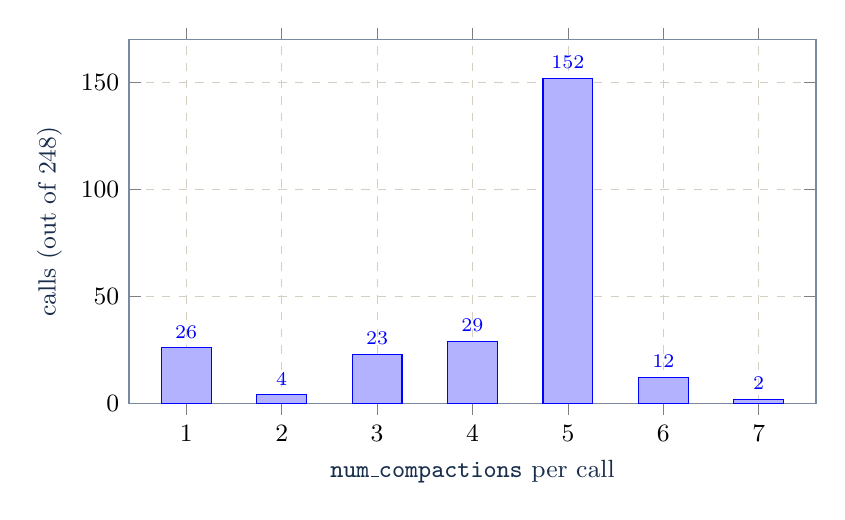
\begin{tikzpicture}
\begin{axis}[
    width=0.85\linewidth, height=6.2cm,
    ybar, bar width=18pt,
    enlarge x limits=0.10,
    ymin=0, ymax=170,
    ylabel={\small calls (out of 248)},
    xlabel={\small \texttt{num\_compactions} per call},
    xtick=data,
    symbolic x coords={1,2,3,4,5,6,7},
    nodes near coords,
    nodes near coords style={font=\scriptsize\color{primary!80!black}},
    tick label style={font=\small},
    label style={font=\small\color{primary!80!black}},
    axis line style={primary!60},
    every axis plot/.append style={fill=primary!30, draw=primary},
    grid=major, grid style={line width=0.2pt, color=rule, dashed},
]
\addplot coordinates {
    (1,26) (2,4) (3,23) (4,29) (5,152) (6,12) (7,2)
};
\end{axis}
\end{tikzpicture}
\caption{Distribution of \sym{num\_compactions}. The mode is 5 (152 calls, 61.3\%): memtable flush plus four non-empty levels.}
\label{fig:hist}
\end{figure}

\begin{itemize}[leftmargin=1.4em,itemsep=2pt]
    \item $\sym{nc}=1$ (26 calls): idle calls where only the memtable flush ran.
    \item $\sym{nc}=5$ (152 calls, 61.3\%): the workload kept L0--L3 populated for most of its run.
    \item The 0.824 compression ratio confirms that compaction effectively removed stale data (17.6\% reduction).
\end{itemize}

\subsection{Representative patterns}

\begin{table}[h!]
\centering
\caption{Pattern families observed in \texttt{compaction\_stats.txt}.}
\label{tab:patterns}
\renewcommand{\arraystretch}{1.2}
\small
\begin{tabularx}{\linewidth}{@{}lXl@{}}
\toprule
\textbf{Line (sample)} & \textbf{What happened} & \textbf{Count} \\
\midrule
\sym{1; 0; 0; 0; 0}          & DB was empty; only the flush ran.                                   & 26 \\
\sym{1; 1; 1; 0; 0}          & One L0 file after flush; no further work.                           & several \\
\sym{5; 2; 1; <r>; <w>}      & Flush + four levels touched; L0--L3 had data.                       & 152 \\
\sym{4; 2; 4; 39649; 45379}  & Inversion: L1 overlap files rewritten alongside L0 input.           & --- \\
\bottomrule
\end{tabularx}
\end{table}

\subsection{Sanity checks}
\begin{itemize}[leftmargin=1.4em,itemsep=2pt]
    \item \sym{num\_compactions} is in $[1, 7]$ for every line, matching the loop bound at \codref{db/db\_impl.cc}{1640}.
    \item \sym{output\_files == 0} only when \sym{input\_files == 0}.
\end{itemize}

\vspace{1em}
\begin{center}
{\color{primary}\rule{0.4\linewidth}{0.6pt}}\\[0.4em]
{\small\itshape\color{primary!70!black}End of report.}
\end{center}

\end{document}
